% Compile with: pdflatex -shell-escape rs2013.tex
\documentclass[xcolor=dvipsnames,red]{beamer}
\usepackage{minted}
\usepackage{latexsym}
\usepackage{amsmath, amsthm}
\usepackage{amsfonts}
\usepackage{amssymb}
\usepackage{amsxtra}
\usepackage{bm}
\usepackage{algorithm}
\usepackage{algpseudocode}
\usetheme{Copenhagen}
\setbeamertemplate{bibliography item}[text]

\title{RedSnake Philly 2013}
\date{}

\begin{document}

%---- title page ----
\begin{frame}[plain]
\titlepage
\vspace{-2 cm}
\begin{center}

\includegraphics[width=.4\textwidth]{imgs/rs-logo-2.png}
\end{center}
\end{frame}

%---- Thanks to sponsors ----
\begin{frame}
\frametitle{Big thanks to our sponsors!}

\begin{columns}
\begin{column}{.33\textwidth}

\includegraphics[width=1\textwidth]{imgs/seer.png}\\
\vspace{.5 cm}

\includegraphics[width=1\textwidth]{imgs/relay.jpg}\\
\vspace{.5 cm}

\includegraphics[width=.75\textwidth]{imgs/new_york_life.jpg}
\end{column}

\begin{column}{.33\textwidth}

\includegraphics[width=1\textwidth]{imgs/monetate.png}\\
\vspace{.5 cm}

\includegraphics[width=1\textwidth]{imgs/jobspring.png}\\
\vspace{.5 cm}

\includegraphics[width=1\textwidth]{imgs/love_park_robotics.png}
\end{column}

\begin{column}{.33\textwidth}

\includegraphics[width=1\textwidth]{imgs/sig.png}\\
\vspace{.5 cm}

\includegraphics[width=.75\textwidth]{imgs/basho.png}\\
\vspace{.5 cm}

\includegraphics[width=1\textwidth]{imgs/mashion.png}\\
\vspace{.5 cm}

\includegraphics[width=1\textwidth]{imgs/critter_case.png}
\end{column}
\end{columns}
\end{frame}

%---- Thanks to Mike D. ----
\begin{frame}
\frametitle{Big thanks to our brewmaster}
%% \begin{center}
%% 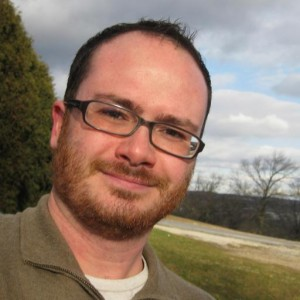
\includegraphics[width=.4\textwidth]{imgs/miked.jpg}
%% \end{center}
\begin{columns}
\begin{column}{.5\textwidth}
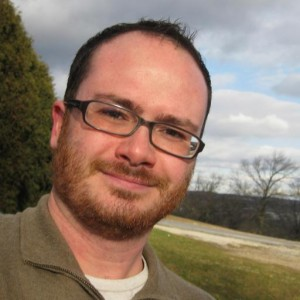
\includegraphics[width=1\textwidth]{imgs/miked.jpg}
\end{column}
\begin{column}{.5\textwidth}
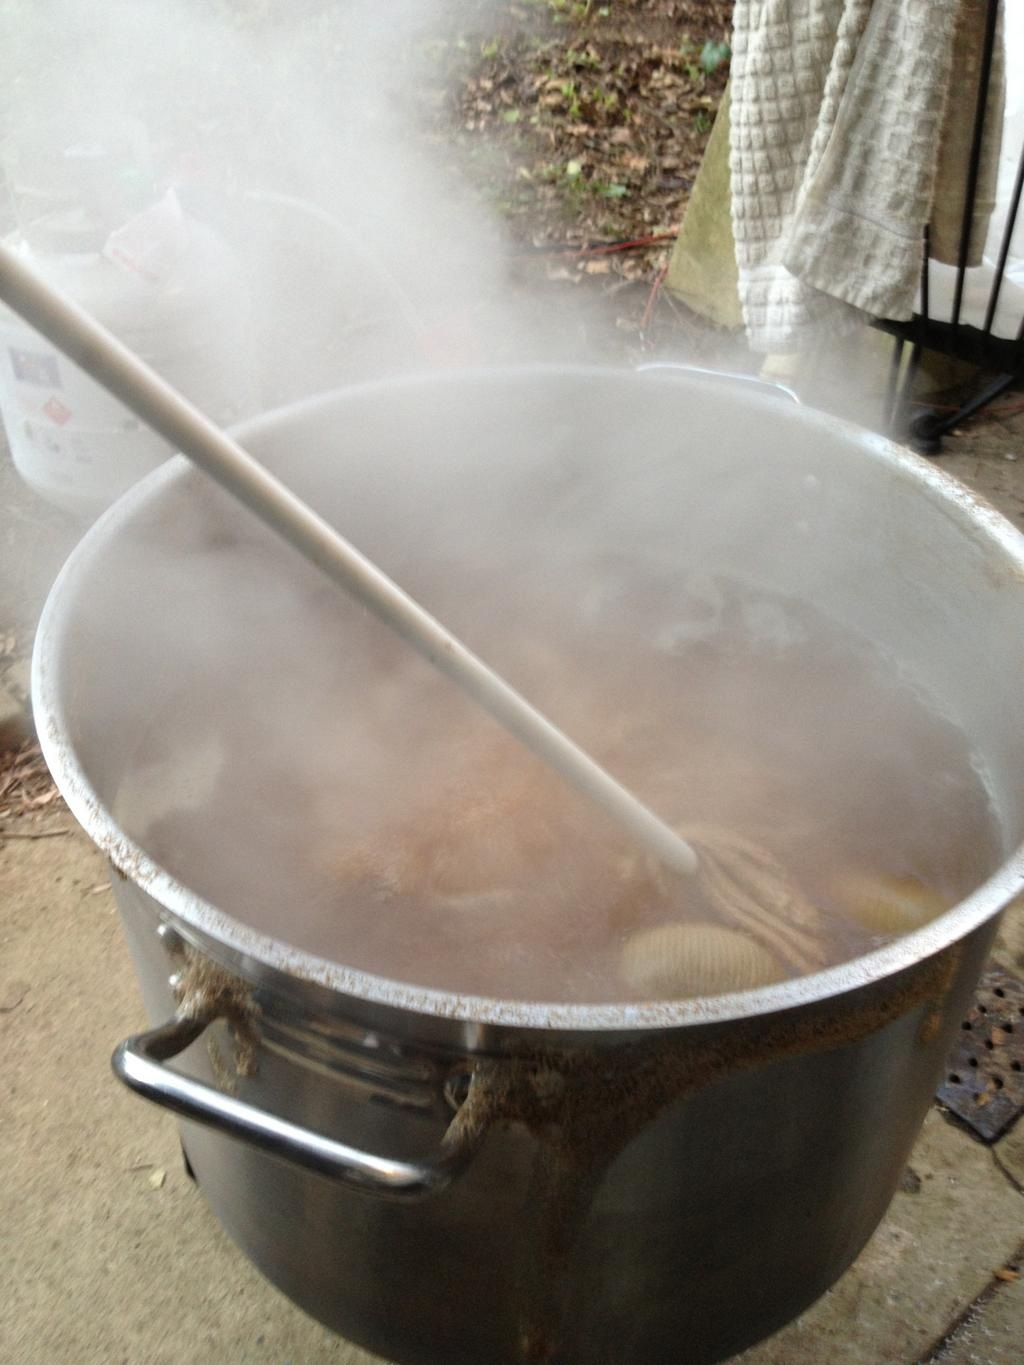
\includegraphics[width=1\textwidth]{imgs/brew.JPG}
\end{column}
\end{columns}
\end{frame}

%---- Goals ----
\begin{frame}
\frametitle{RedSnake Philly Manifesto}
\begin{enumerate}
\item To be the premier technical event for hardcore programmers in Philadelphia
\item To inspire and provide an environment of learning to those who are new to programming
\item To introduce Philadelphia's top companies to Philadelphia's top programmers
\item To raise national recognition for Philadelphia's tech community and
  attract top talent to the city
\end{enumerate}
\end{frame}

%---- Agenda ----
\begin{frame}
\frametitle{Tonight's agenda}
\begin{columns}

\begin{column}{.35\textwidth}
3:30 PM - 4:30 PM\\
4:30 PM - 5:30 PM\\
5:30 PM - 5:40 PM\\
5:40 PM - 7:00 PM\\
7:10 PM - 7:20 PM\\
7:20 PM - 8:20 PM\\
8:20 PM - 9:30 PM\\
9:31 PM
\end{column}

\begin{column}{.65\textwidth}
Happy Hour\\
Dinner\\
(you are here)\\
Technical and Sponsor Talks\\
Coffee, Desserts, and Giveaways\\
Technical and Sponsor Talks\\
Even Happier Hour\\
You Leave
\end{column}

\end{columns}
\end{frame}

%---- Speakers ----
\begin{frame}
\frametitle{Tonight's Speakers}

\begin{columns}
\begin{column}{.25\textwidth}
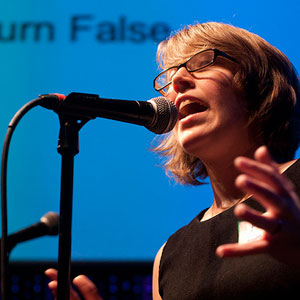
\includegraphics[width=.75\textwidth]{imgs/pam_selle.jpg}\\
\vspace{.2 cm}
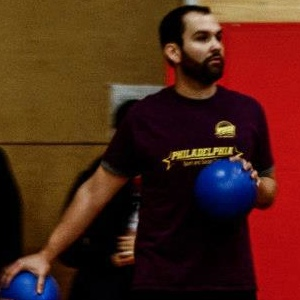
\includegraphics[width=.75\textwidth]{imgs/hcastro.jpg}\\
\vspace{.2 cm}
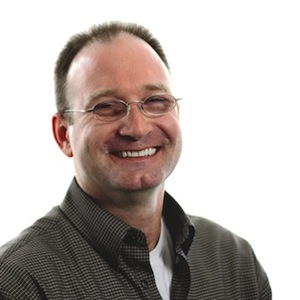
\includegraphics[width=.75\textwidth]{imgs/jeff_persch.jpg}
\end{column}

\begin{column}{.25\textwidth}
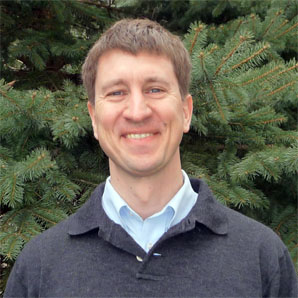
\includegraphics[width=.75\textwidth]{imgs/scott_determan.jpg}\\
\vspace{.2 cm}
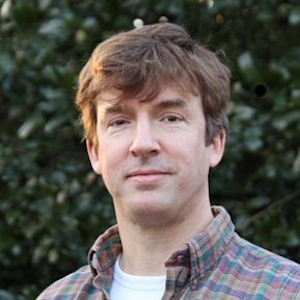
\includegraphics[width=.75\textwidth]{imgs/tom_adelman.jpg}\\
\vspace{.2 cm}
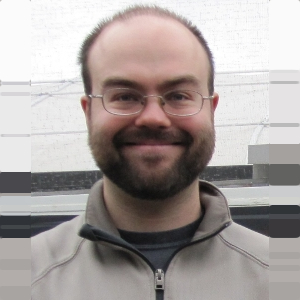
\includegraphics[width=.75\textwidth]{imgs/david_richardson.jpg}
\end{column}

\begin{column}{.25\textwidth}
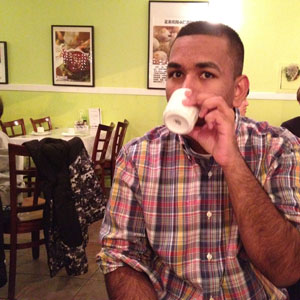
\includegraphics[width=.75\textwidth]{imgs/jearvon_dharrie.jpg}\\
\vspace{.2 cm}
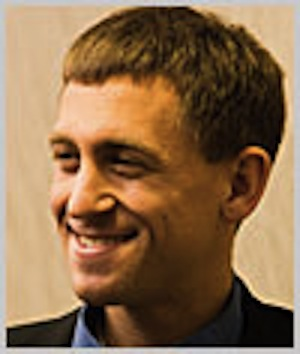
\includegraphics[width=.75\textwidth]{imgs/dimarco.jpg}\\
\vspace{.2 cm}
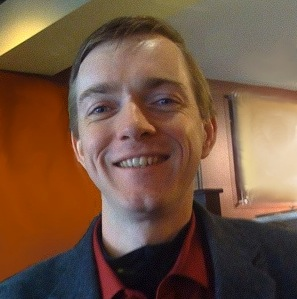
\includegraphics[width=.75\textwidth]{imgs/kyle_burton.jpg}
\end{column}

\begin{column}{.25\textwidth}
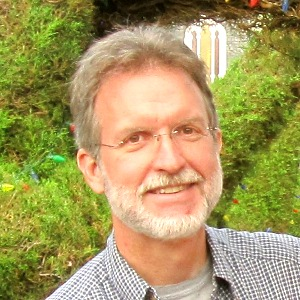
\includegraphics[width=.75\textwidth]{imgs/dan_williams.jpg}\\
\vspace{.2 cm}
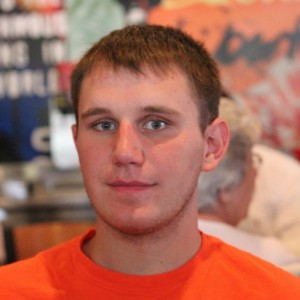
\includegraphics[width=.75\textwidth]{imgs/justin_campbell.jpg}
\end{column}
\end{columns}

\end{frame}

%---- Speaker Logistics ----
\begin{frame}
\frametitle{Speaker Logistics}
\begin{enumerate}
\item You get {\em exactly} 10 minutes
\item I will signal you at 5 min, 3 min, 1 min, 10 sec, GONG
\item Tech talk + sponsor talk gets a total of 20 min (split it up as you wish)
\item If you do the above, you will get two sets of 5-3-1-10-GONG
\item When you are on-deck, get ready for a fast transition
\end{enumerate}

Any Questions?
\end{frame}

%---- General Logistics ----
\begin{frame}
\frametitle{General Logistics}
\begin{enumerate}
\item There are seats upstairs if you did not get a pew
\item Try to refrain from using laptops, tweet with your phone
\item Bathrooms are located at... (Chris?)
\item Beer is in the back
\item Coffee and dessert will be served in the back at break
\end{enumerate}

Any Questions?
\end{frame}

%----Go ----
\begin{frame}[plain]
\titlepage
\vspace{-2 cm}
\begin{center}

\includegraphics[width=.4\textwidth]{imgs/rs-logo-2.png}
\end{center}
\end{frame}

\end{document}
